\section{Techniken}

\subsection{Divide and Conquer}
Divide and Conquer ist vor allem bekannt als Paradigma von rekursiven
Algorithmen.
Ein Problem wird zunächst in kleinere Teilprobleme aufgeteilt (\emph{divide}).
Diese werden rekursiv gelöst (\emph{conquer}) und anschließend zur der Lösung
des ursprünglichen Problems zusammengesetzt (\emph{combine}).

Das Aufteilen und wieder Zusammensetzen ist meist mit Aufwand verbunden.
Entweder wird so geteilt, dass sich die Lösungen der Teilprobleme sehr einfach
kombinieren lassen. Ein Algorithmus, der diesen Ansatz verwendet, ist
Quicksort (Algorithmus \ref{alg:quicksort}).
Es wird ein Pivotelement gewählt und die zu sortierende Liste anhand diesem
aufgeteilt, so dass das Zusammenführen durch einfache Konkatenation möglich
ist.
Die zweite Möglichkeit, eine einfache Aufteilung zu verwenden und das
die Arbeit beim Zusammenführen zu erledigen, verwendet Mergesort (Algorithmus
\ref{alg:mergesort}).
Die Eingabe wird in der Mitte geteilt, beide Teilarrays sortiert und
anschließend zusammengeführt.

\begin{algorithm}
    \caption{Quicksort \cite[S.171]{cormen}}
    \label{alg:quicksort}
    \begin{algorithmic}[1]
    \Require Ein Array $A$ mit den Indices $p$ und $r$.
    \Ensure Das Array $A$ sortiert zwischen $p$ und $r$.
    \If {$p < r$}
        \State $q \gets \textsc{Partition}(A,r,p)$
        \State $\textsc{Quicksort}(A, p, q - 1)$
        \State $\textsc{Quicksort}(A, q + 1, r)$
    \EndIf
    \end{algorithmic}
\end{algorithm}

\begin{algorithm}
    \caption{Mergesort \cite[S.34]{cormen}}
    \label{alg:mergesort}
    \begin{algorithmic}[1]
    \Require Ein Array $A$ mit den Indices $p$ und $r$.
    \Ensure Das Array $A$ sortiert zwischen $p$ und $r$.
    \If {$p < r$}
        \State $q \gets \lfloor (p + r) / 2 \rfloor$
        \State $\textsc{Mergesort}(A, p, q)$
        \State $\textsc{Mergesort}(A, q + 1, r)$
        \State $\textsc{Merge}(A, p, q, r)$
    \EndIf
    \end{algorithmic}
\end{algorithm}

In beiden Beispielalgorithmen wird die Prozedur zweimal nacheinander rekursiv
aufgerufen.
Die Aufrufe bearbeiten verschiedene Teile des Arrays.
Das naheliegendste Verfahren, um die Algorithmen zu parallelisieren, wäre es,
die beiden rekursiven Aufrufe parallel auszuführen.
Eine Aufteilung der Eingabe in $p$ Teile, die anschließend von $p$ Prozessoren
bearbeitet werden wäre ebenso möglich.
Allerdings ist ein schneller Algorithmus abhängig von der effizienten Ausführung
des ersten und des dritten Schrittes.
\cite[S.30ff.]{cormen}
\cite[S.56ff.]{jaja}

\begin{table}
    \centering
    \begin{tabularx}{\textwidth}{|l|X|X|}
        \hline
        & Quicksort & Mergesort \\ \hline
        Divide  &
        Wahl eines Pivotelements; \newline
        aufteilen in zwei Teilarrays anhand diesem. &
        Teilung des Arrays in zwei Hälften. \\
        \hline
        Conquer &
        Rekursives Sortieren beider Teile. &
        Rekursives Sortieren beider Teile. \\
        \hline
        Combine &
        Konkatenation der sortierten Teilarray. &
        Zusammenfügen (Merge) der sortieren Teilarrays. \\
        \hline
    \end{tabularx}
    \caption{Divide and Conquer in Quicksort und Mergesort}
    \label{tab:dac}
\end{table}

\subsection{Pointer Jumping}
Pointer Jumping wird bei Problemen, die auf Graphen basieren angewandt.
Die Kanten eines Graphen werden in Datenstrukturen als Zeiger auf einen anderen
Knoten gespeichert.
Solange es möglich ist, die Daten effizient in einer geeigneten Struktur zu
speichern, kann die Technik auch auf Probleme angewandt werden, die an sich
keine Verbindung zu Graphen haben.
Das Pointer Jumping erlaubt parallele Verarbeitung von Daten, die zum Beispiel
in gerichteten Bäumen gespeichert sind.
Zeigen die Kanten zu dem Vater eines Knoten; von den Blättern in Richtung
Wurzel, spricht man auch von einem \emph{In-Tree}.
Ein einfaches Beispiel ist die Suche nach den Wurzeln in einem Wald.
%
\begin{problem}
    Sei $F$ ein Wald aus einer Menge an In-Trees.
    Gegeben ist ein Knoten $j$ in einem der Bäume in $F$.
    Der Wald enthält $n$ Knoten und ist angegeben als ein Array $P$ der Länge
    $n$.
    $P(i)$ enthalte den Vater von $i$.
    Ist $w$ eine Wurzel in $F$, so gelte $P(w) = w$.
    Gesucht ist die Wurzel des Baumes, der den Knoten $j$ enthält.
\end{problem}
%
In jedem Schritt wird der Vater eines Knoten auf den Vater des alten
Vaterknoten gesetzt.
Die Distanz zwischen einem bestimmten Knoten $i$ und $P(i)$ verdoppelt sich bei
jeder Anwendung der Technik, es sei denn $P(i)$ zeigt auf eine Wurzel.
In Abbildung \ref{fig:pointerjumping} ist die Anwendung des Algorithmus
\ref{alg:pointerjumping} auf einen Wald bestehend aus einem verzweigten und
einem linearen Baum zu sehen.
%
\begin{algorithm}
    \caption{Pointer Jumping \cite[S.52]{jaja}}
    \label{alg:pointerjumping}
    \begin{algorithmic}[1]
    \Require Ein Wald aus In-Trees jeweils mit einer Schleifer an der Wurzel.
        Jede Kante zwischen den $n$ Knoten ist als Tupel $(i, P(i))$ mit
        $1 \leq i \leq n$ durch ein Array $P$ definiert.
    \Ensure Für jeden Knoten $i$ die Wurzel $S(i)$ des $i$ beinhaltenden
        Baumes in einem Array $S$.
    \ParDo {$1 \leq i \leq n$}
        \State $S(i) \gets P(i)$
        \While {$S(i) \neq S(S(i))$}
            \State $S(i) \gets S(S(i))$
        \EndWhile
    \EndParDo
    \end{algorithmic}
\end{algorithm}
%
\begin{figure}
    \centering
    \subfloat[]{% pointer jumping on a forest of two trees
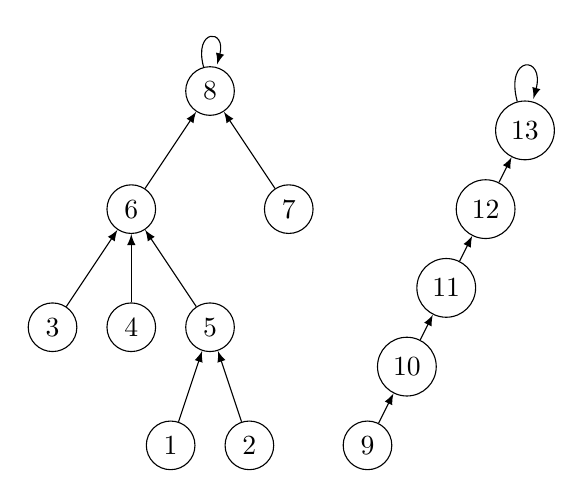
\begin{tikzpicture}
    [
        ->,>=latex,
        vertex/.style={circle, draw, scale=1, minimum size=3ex,},
        edge/.style={-latex,},
    ]

    % t1
    \node (1) at (1.5,0) [vertex] {$1$};
    \node (2) at (2.5,0) [vertex] {$2$};
    \node (3) at (0,1.5) [vertex] {$3$};
    \node (4) at (1,1.5) [vertex] {$4$};
    \node (5) at (2,1.5) [vertex] {$5$};
    \node (6) at (1,3)   [vertex] {$6$};
    \node (7) at (3,3)   [vertex] {$7$};
    \node (8) at (2,4.5) [vertex] {$8$};

    \path
    (1) edge (5)
    (2) edge (5)
    (3) edge (6)
    (4) edge (6)
    (5) edge (6)
    (6) edge (8)
    (7) edge (8)
    (8) edge [loop above] (8);

    % t2
    \node (9)  at (4,0)   [vertex] {$9$};
    \node (10) at (4.5,1) [vertex] {$10$};
    \node (11) at (5,2)   [vertex] {$11$};
    \node (12) at (5.5,3) [vertex] {$12$};
    \node (13) at (6,4)   [vertex] {$13$};

    \path
    (9)     edge    (10)
    (10)    edge    (11)
    (11)    edge    (12)
    (12)    edge    (13)
    (13) edge [loop above] (13);

\end{tikzpicture}
}
    \subfloat[]{% pointer jumping on a forest of two trees
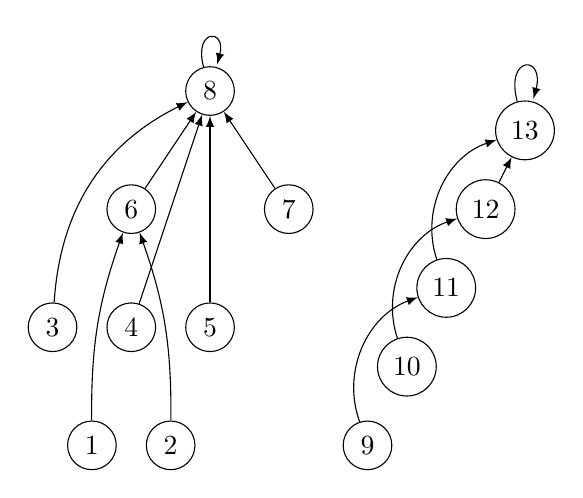
\begin{tikzpicture}
    [
        ->,>=latex,
        vertex/.style={circle, draw, scale=1, minimum size=3ex,},
        edge/.style={-latex,},
    ]

    % t1
    \node (1) at (0.5,0) [vertex] {$1$};
    \node (2) at (1.5,0) [vertex] {$2$};
    \node (3) at (0,1.5) [vertex] {$3$};
    \node (4) at (1,1.5) [vertex] {$4$};
    \node (5) at (2,1.5) [vertex] {$5$};
    \node (6) at (1,3)   [vertex] {$6$};
    \node (7) at (3,3)   [vertex] {$7$};
    \node (8) at (2,4.5) [vertex] {$8$};

    \path
    (1) edge [bend left=10]     (6)
    (2) edge [bend right=10]    (6)
    (3) edge [bend left]        (8)
    (4) edge                    (8)
    (5) edge                    (8)
    (6) edge                    (8)
    (7) edge                    (8)
    (8) edge [loop above]       (8);

    % t2
    \node (9)  at (4,0)   [vertex] {$9$};
    \node (10) at (4.5,1) [vertex] {$10$};
    \node (11) at (5,2)   [vertex] {$11$};
    \node (12) at (5.5,3) [vertex] {$12$};
    \node (13) at (6,4)   [vertex] {$13$};

    \path
    (9)     edge [bend left=45] (11)
    (10)    edge [bend left=45] (12)
    (11)    edge [bend left=45] (13)
    (12)    edge                (13)
    (13)    edge [loop above]   (13);

\end{tikzpicture}
}
    \newline
    \subfloat[]{% pointer jumping on a forest of two trees
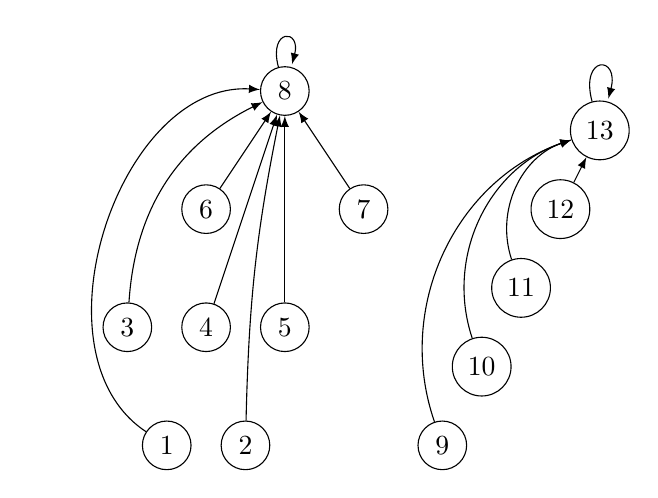
\begin{tikzpicture}
    [
        ->,>=latex,
        vertex/.style={circle, draw, scale=1, minimum size=3ex,},
        edge/.style={-latex,},
    ]

    % t1
    \node (1) at (0.5,0) [vertex] {$1$};
    \node (2) at (1.5,0) [vertex] {$2$};
    \node (3) at (0,1.5) [vertex] {$3$};
    \node (4) at (1,1.5) [vertex] {$4$};
    \node (5) at (2,1.5) [vertex] {$5$};
    \node (6) at (1,3)   [vertex] {$6$};
    \node (7) at (3,3)   [vertex] {$7$};
    \node (8) at (2,4.5) [vertex] {$8$};

    \path
    (1) edge [bend left=75]     (8)
    (2) edge [bend left=5]      (8)
    (3) edge [bend left]        (8)
    (4) edge                    (8)
    (5) edge                    (8)
    (6) edge                    (8)
    (7) edge                    (8)
    (8) edge [loop above]       (8);

    % t2
    \node (9)  at (4,0)   [vertex] {$9$};
    \node (10) at (4.5,1) [vertex] {$10$};
    \node (11) at (5,2)   [vertex] {$11$};
    \node (12) at (5.5,3) [vertex] {$12$};
    \node (13) at (6,4)   [vertex] {$13$};

    \path
    (9)     edge [bend left=45] (13)
    (10)    edge [bend left=45] (13)
    (11)    edge [bend left=45] (13)
    (12)    edge                (13)
    (13)    edge [loop above]   (13);

\end{tikzpicture}
}
    \caption{Ausführung von Algorithmus \ref{alg:pointerjumping}
    (nach \cite[S.54]{jaja})}
    \label{fig:pointerjumping}
\end{figure}
\cite[S.52ff]{jaja}
